
\documentclass[12pt]{article}

\title{Proyección del número de muertes totales para los paises de México, Canada, Brasil y Estados Unidos para el año 2020, sin considerar el Covid.}

\date{}
\usepackage{braket}
\usepackage{bbold}
\usepackage{amsmath,amsfonts,amssymb,amsthm,booktabs}
\usepackage[margin=1.0in]{geometry}
\usepackage{graphicx}
\usepackage{chngcntr}
\usepackage{floatrow}
\usepackage{chngcntr}
\usepackage{hyperref}
\usepackage[spanish]{babel}
\usepackage[svgnames]{xcolor}
\usepackage{commath}
\usepackage{floatrow}
\floatsetup[table]{capposition=top}
\DeclareRobustCommand{\bbone}{\text{\usefont{U}{bbold}{m}{n}1}}

\DeclareMathOperator{\EX}{\mathbb{E}}% expected val
\renewcommand{\spanishtablename}{Cuadro}
\usepackage{listings}
\usepackage[%
    font={small,sf},
    labelfont=bf,
    format=hang,    
    format=plain,
    margin=0pt,
    width=0.8\textwidth,
]{caption}
\usepackage[list=true]{subcaption}
\lstset{language=R,
    basicstyle=\small\ttfamily,
    stringstyle=\color{DarkGreen},
    otherkeywords={0,1,2,3,4,5,6,7,8,9},
    morekeywords={TRUE,FALSE},
    deletekeywords={data,frame,length,as,character},
    keywordstyle=\color{blue},
    commentstyle=\color{DarkGreen},
}

\counterwithin{figure}{section}
\renewcommand*{\figureautorefname}{Figura}


\usepackage[backend=biber]{biblatex}
\addbibresource{ref.bib}
\renewcommand{\baselinestretch}{1.5}
\begin{document}
	\maketitle
	\begin{center}


\textbf{ }

\centerline{Alumno: } 
\centerline{Joaquín Arturo Velarde Moreno}


	\end{center}

\section{Introducción}
Desde que en marzo de 2020 se dieron los primeros contagios por el Sars Covid 19 en nuestro país, se ha venido afirmando por expertos en Salud, estadísticos y medios de comunicación que en México el número de infectados por esta nueva enfermedad ha sido mayor al reportado por las cifras oficiales de la Secretaría de salud. Recientemente, incluso el propio subsecretario, Dr. López Gatell, y vocero oficial del gobierno federal en esta problemática, reconoció que el número de contagios podría ser mayor e inconmensurable debido a que no se ha hecho el suficiente número de pruebas tanto a enfermos como post mortem.
¿Cómo se podría llegar a conocer el número real de fallecidos por este nuevo virus? aún más, ¿se puede hacer un estimado del número de fallecimientos que esta pandemia causará en México? 
En la presente investigación nos proponemos elaborar, mediante una proyección probabilística, el número de muertes por exceso debido al Covid para el año 2020, tomando en cuenta el número total de fallecidos que son reportados oficialmente por año a partir del 2010, a fin de contrastar los resultados con los reportes oficiales del Covid para ver la correspondencia.

Nos hemos propuesto, además, realizar las proyecciones de los países de Estados Unidos de Norteamérica y Canadá para hacer un comparativo con nuestro país, ya que con dichos países nos unen fuertes lazos económicos, sobre todo a partir de la firma del T-MEC \cite{MEC}.  
También hemos considerado en este análisis a Brasil ya que es un país que se encuentra entre los más poblados de América Latina como el nuestro. 

\section{Método}

Para este trabajo, primeramente se buscaron los datos de los países mencionados que se reportan por los gobiernos a la página web DatosMacro \cite{datosmacro}
Y para el caso de México, se consultaron las cifras que reporta INEGI en su página oficial\cite{inegi}. 
Con los datos obtenidos se elaboraron las gráficas mediante el software R \cite{rproject} para poder visualizar las relaciones entre las defunciones y el año de cada uno de los países mencionados.
Con los resultados se obtuvieron ciertas propiedades de los datos, tales como la media , la varianza y la desviación estándar, para poder calcular las ecuaciones necesarias y hacer la predicción para el año 2020.
Las ecuaciones usadas fueron la regresión lineal y la correlación de Pearson. 
Tomando en cuenta el resultado de la proyección, se compara con los otros países para ver la evolución de cada uno.


\subsection{Datos oficiales}
En el Cuadro 1, se muestran los datos de muertes anuales de cada uno de los países seleccionados.  
Se puede observar en ese cuadro, que el número de fallecimientos de cada país se relaciona con el número total de población de cada uno de ellos.
Dado que la página consultada para  los países extranjeros  no reporta el año 2019 , también se elaboró la proyección del año faltante para poder compararlos con México.
En el caso de México se pudo obtener hasta 2019, siendo los siguientes los casos oficiales.




\begin{table}[H]
\begin{center}
\caption{Tabla de defunciones de Brasil, Canadá y USA en los años 2010 - 2018.}
\begin{tabular}{c|rrrrr}
\multicolumn{1}{l}{} & \textbf{Brasil} & \textbf{Canadá} & \textbf{USA} & \textbf{México}\\
\hline
\textbf{2010}        & 1,178,116           & 240,295             & 2,473,239                  & 592,018\\
\textbf{2011}  & 1,193,583           & 247,608             & 2,516,058          &   590,693         \\
\textbf{2012}    & 1,210,911          & 252,242              & 2,544,015           &  602,354      \\
\textbf{2013}    & 1,229,425          & 252,245            & 2,597,623            &  623,599     \\
\textbf{2014}    & 1,249,643         & 258,362           & 2,624,007             &  633,641 \\
\textbf{2015}    & 1,271,725           & 264,017            & 2,708,367              & 655,688   \\
\textbf{2016}    & 1,294,746          & 266,785             & 2,744,322               & 685,766 \\
\textbf{2017}    & 1,325,564         & 273,668            & 2,810,166             &  703,047   \\
\textbf{2018}    & 1,351,496           & 284,854             & 2,815,227  &  722,611   \\
\textbf{2019}    & N/A           & N/A             & N/A  &  747,784   \\


\end{tabular}
\label{mortalidadBrasil}
\end{center}
\end{table}




\subsection{Métodos estadísticos}
Antes de empezar, es necesario establecer ciertos conceptos para que nos faciliten el cálculo del número de defunciones del año 2020,
el primero de estos es la media:
\[ \mu = \frac{\Sigma x_{i}}{n} .\]
Donde:
\begin{itemize}
	\item $x$ = vector de elementos,
	\item $x_{i}$ = elemento del vector,
	\item $n$ = número total de elementos.

\end{itemize}
El segundo es la varianza:
\[ \sigma^{2} = \frac{\Sigma (x_{i}-\mu)^{2}}{n} .\]
el tercero la desviación estándar:
\[ \sigma = \sqrt{\sigma^{2}} = \sqrt{\frac{\Sigma (x_{i}-\mu)^{2}}{n}}.\]

En las figuras \ref{fig:casoMexico},\ref{fig:casoCanada},\ref{fig:casoUsa},\ref{fig:casoBrasil}, se grafican la incidencia anual de defunciones en cada uno de los países analizados. 
Como se puede observar, el número de fallecidos ha ido aumentando cada año, por lo que hay una relación entre el año y número de defunciones. 


\begin{figure}[H]
\centering{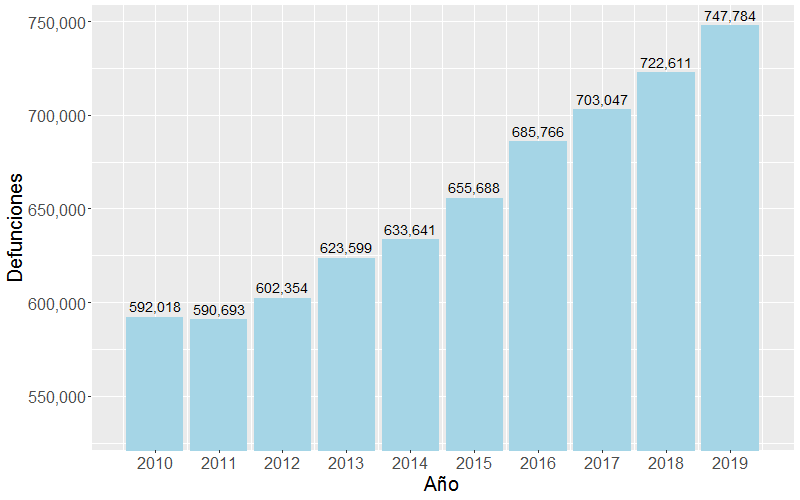
\includegraphics[width=0.8\textwidth]{Figuras/DefuncionesAnualesMexico.png}}%
\hfill
\caption{Defunciones de México por año.}
\label{fig:casoMexico}
\end{figure}

\begin{figure}[H]
\centering{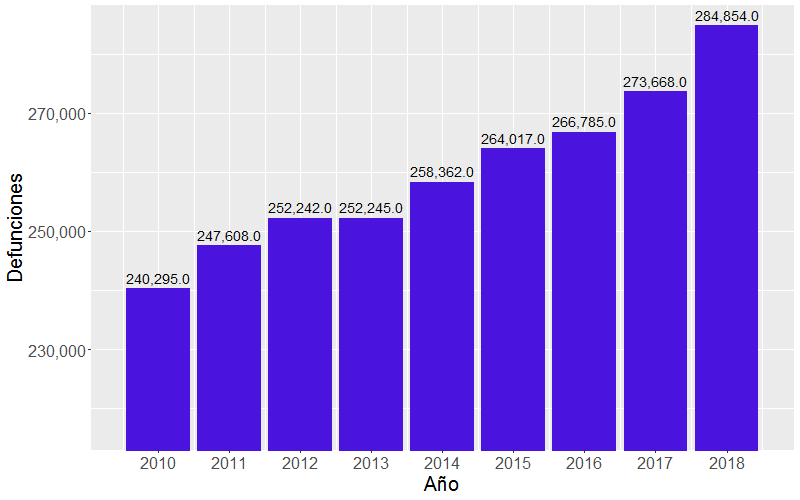
\includegraphics[width=0.8\textwidth]{Figuras/DefuncionesAnualesCanada.png}}%
\hfill
\caption{Defunciones de Canadá por año.}
\label{fig:casoCanada}
\end{figure}

\begin{figure}[H]
\centering{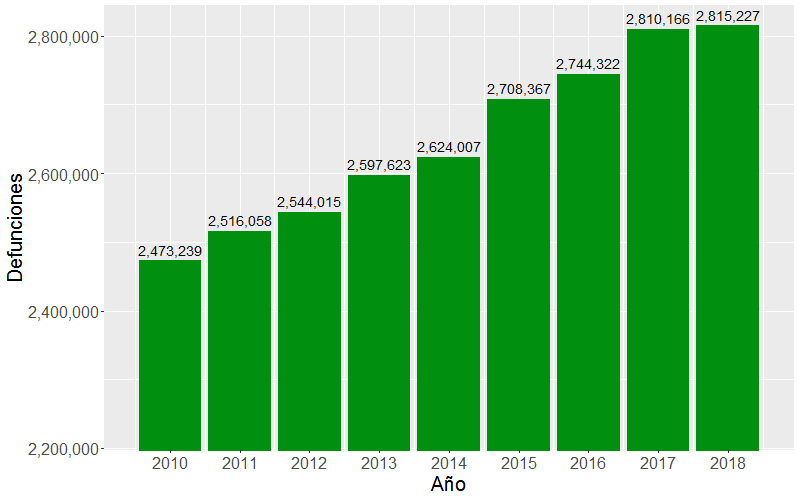
\includegraphics[width=0.8\textwidth]{Figuras/DefuncionesAnualesUSA.png}}%
\hfill
\caption{Defunciones de los Estados Unidos por año.}
\label{fig:casoUsa}
\end{figure}

\begin{figure}[H]
\centering{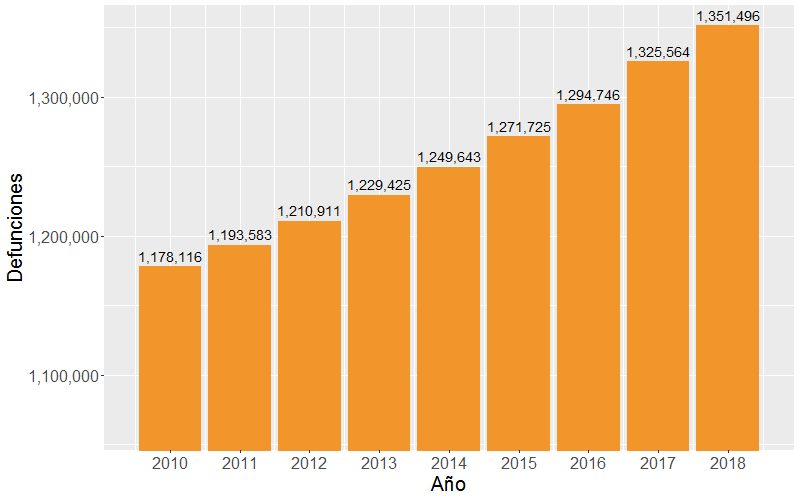
\includegraphics[width=0.8\textwidth]{Figuras/DefuncionesAnualesBrasil.png}}%
\hfill
\caption{Defunciones de Brasil por año.}
\label{fig:casoBrasil}
\end{figure}


Se obtuvo esta relación mediante la correlación de Pearson, la cual a su vez se obtiene por la siguiente expresión y varía entre los rangos de 1 a -1:
\[\ r = \frac{\Sigma\left(x\ \times\ y\right)\ -\ \frac{1}{n}\left(\Sigma x\ \times\Sigma y\right)}{\sqrt{\left(\Sigma x^2-\frac{1}{2}\left(\Sigma x\right)^2\right)\times\left(\Sigma y^2-\frac{1}{2}\left(\Sigma y\right)^2\right)}}.\]

Donde:
\begin{itemize}
	\item $x\ e\ y$ son nuestros datos bivariados,
	\item $n$ es el número de datos.
\end{itemize}
Otra forma de realizar este cálculo es obteniendo  los promedios de cada vector, a los cuales denotaremos como $X\ y\ Y$, la cual se expresa:
\[\ r =  \frac{\Sigma\left(x\ \times\ y\right)}{\sqrt{\Sigma x^2\times\Sigma y^2}}.\]
Donde:
\begin{itemize}
	\item $y$ = $Y - \mu Y$,
	\item $x$ = $X - \mu X$.
\end{itemize}
Para poder visualizar la relación entra ambos vectores, es necesario usar el método de la regresión lineal. Si definimos esta recta como:
\[ y = b + mx .\]
Donde:
\begin{itemize}
	\item $m$ es la pendiente,
	\item $b$ coordenada origen.
\end{itemize}
$m$ esta dada por :
\[ m = r * (\frac{\sigma_{y}}{\sigma{x}}).\]
$b$ es obtenida :
\[ b = \mu_{y}(m * \mu_{x}).\]

Error estándar:
\[ \sigma_{e} = \sqrt{\frac{\Sigma (Y - Y_{p})^{2}}{n}} .\]
Donde:
\begin{itemize}
	\item $n$ número de elementos,
	\item $Y_{p}$ regresión lineal.
\end{itemize}

\section{Resultados}
A continuación se muestran los resultados obtenidos por medio de la regresión lineal para la estimación de las muertes posibles en México para el año 2020 ver figura \ref{fig:RegresionMexico}.
Aunque se observa en la gráfica de regresión lineal 3 puntos un poco fuera de nuestro error estándar, otros 5 caen dentro de nuestro error estándar por lo que la estimación puede ser un número confiable, de aquí obtuvimos el error estándar que es $\pm$ 8892, por lo que los valores esperados estarán en el intervalo [748072,765856].
Donde nuestro valor mínimo es cercano a nuestro valor reportado oficialmente el año anterior.

\begin{figure}[H]
\centering
\subcaptionbox{Regresión lineal para México.}{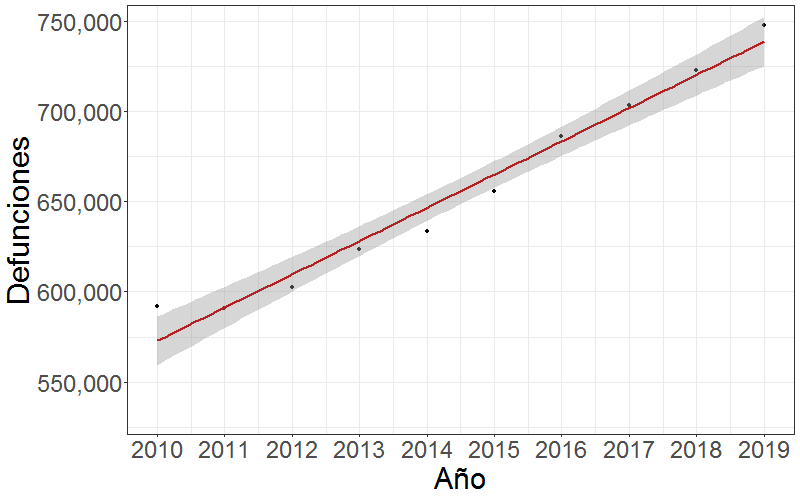
\includegraphics[width=0.4\textwidth]{Figuras/DefuncionesAnualesRegresionMexico.png}}%
\hfill
\subcaptionbox{Media de población que cruza por la recta en México.}{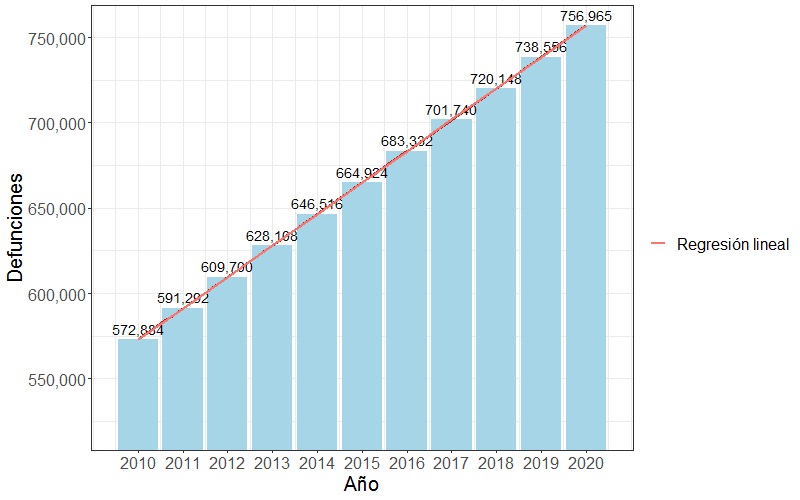
\includegraphics[width=0.6\textwidth]{Figuras/DefuncionesAnualesRegresionFinalMexico.png}}%
\hfill
\caption{Regresión lineal para el país de México junto con la media en 2020.}

\label{fig:RegresionMexico}
\end{figure}   
\hfill

Para el caso de Canadá los resultados obtenidos por medio de la regresión lineal para la estimación de las muertes posibles para este país para el año 2020 se muestran en la figura 3.2.
Aquí que en la gráfica de regresión lineal se ajusta mas a los datos pues los puntos caen todos dentro del error estándar, por lo que la estimación puede ser un número confiable, aquí obtuvimos el error estándar que es $\pm$ 2553, por lo que los valores esperados estarán en el intervalo [287181,292289].


\begin{figure}[H]
\centering
\subcaptionbox{Regresión lineal para Canadá.}{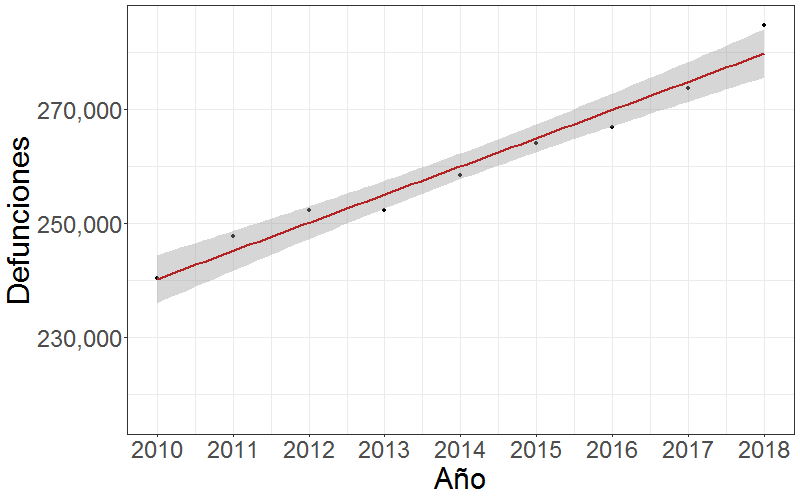
\includegraphics[width=0.4\textwidth]{Figuras/DefuncionesAnualesRegresionCanada.png}}%
\hfill
\subcaptionbox{Media de población que cruza por la recta en Canadá.}{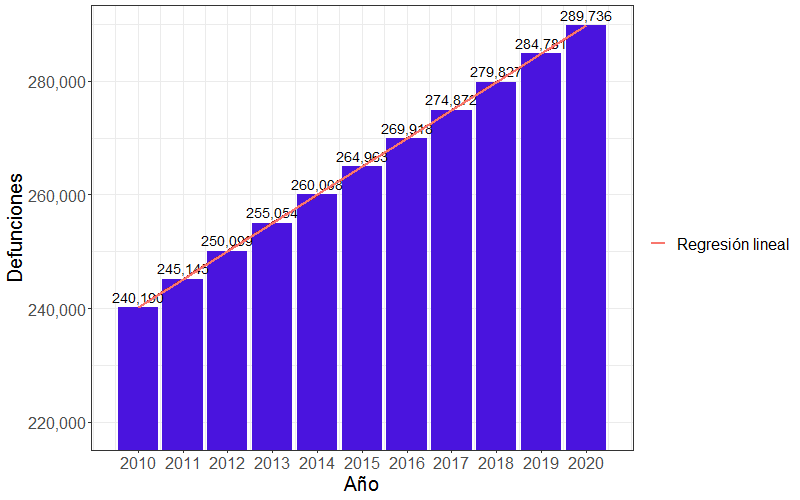
\includegraphics[width=0.6\textwidth]{Figuras/DefuncionesAnualesRegresionFinalCanada.png}}%
\hfill
\caption{Regresión lineal para el país de Canadá junto con la media en 2020.}

\label{fig:RegresionCanada}
\end{figure}   
\hfill

Para el caso de USA la gráfica de regresión abarca muy bien todos los puntos, pero se puede observar que los valores, se alternan año con año por arriba y por debajo de la recta de regresión lineal, por lo que es posible, que el número de muertes para 2019 y 2020, este un poco sobrestimado, aquí esperaríamos que el valor de muertes en Estados Unidos que estuviera en el rango mínimo de nuestro error estándar que fue de $\pm$ 14722. Así que si el rango fue [2909554,2938999] esperaríamos que Estados Unidos estaría en los 2,909,554.


\begin{figure}[H]
\centering
\subcaptionbox{Regresión lineal para USA.}{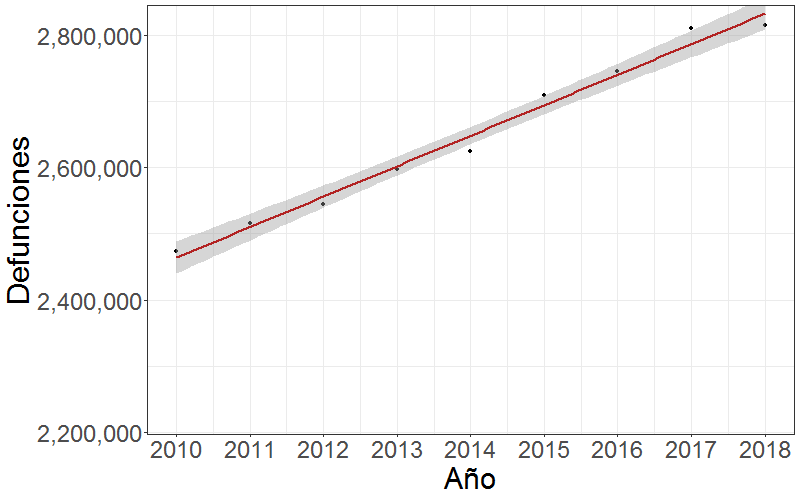
\includegraphics[width=0.4\textwidth]{Figuras/DefuncionesAnualesRegresionUSA.png}}%
\hfill
\subcaptionbox{Media de población que cruza por la recta en USA.}{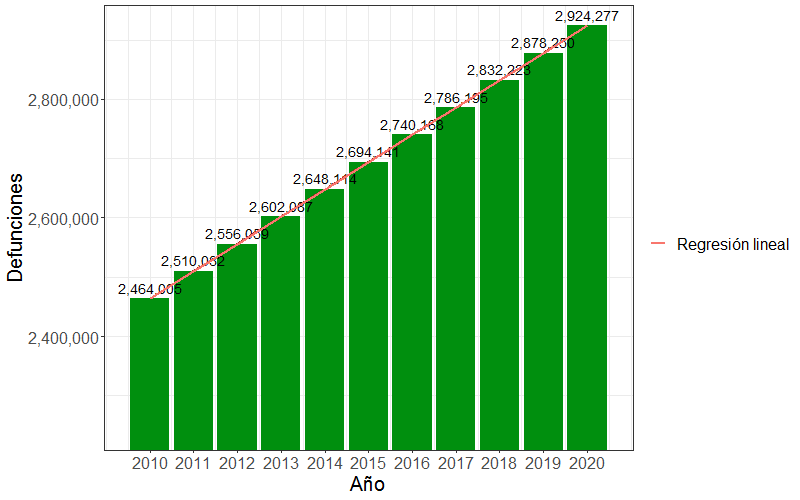
\includegraphics[width=0.6\textwidth]{Figuras/DefuncionesAnualesRegresionFinalUSA.png}}%
\hfill
\caption{Regresión lineal para el país de USA junto con la media en 2020.}

\label{fig:RegresionUSA}
\end{figure}   
\hfill

También la regresión lineal para Brasil muestra un buen comportamiento y se apega a los datos aunque muestra una tendencia creciente en los últimos 2 años que se tienen de datos, por lo que nuestro número estimado podría estar por debajo del número real.
Para el error estándar aquí calculamos $\pm$ 5834 y el valor central en un 
1,386,078 así que los valores estarían en el rango de [1380243,1391912] por lo dicho anteriormente esperaríamos que el número de muertes este en 1,391,912.\\


\begin{figure}[H]
\centering
\subcaptionbox{Regresión lineal para Brasil.}{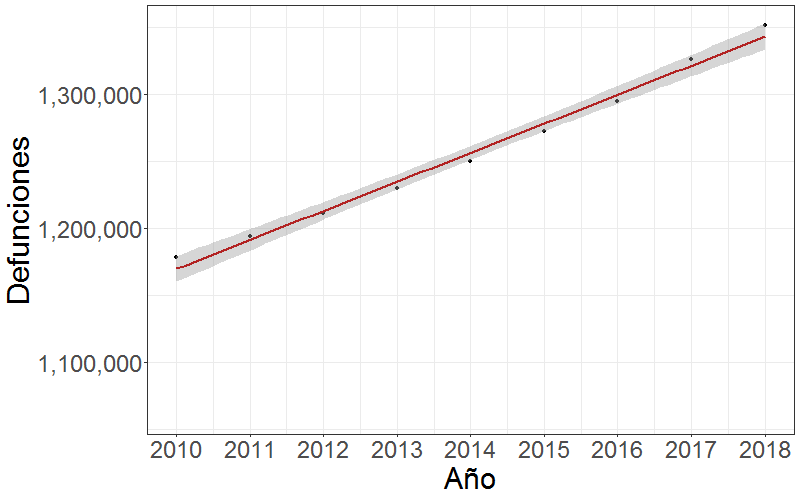
\includegraphics[width=0.4\textwidth]{Figuras/DefuncionesAnualesRegresionBrasil.png}}%
\hfill
\subcaptionbox{Media de población que cruza por la recta en Brasil.}{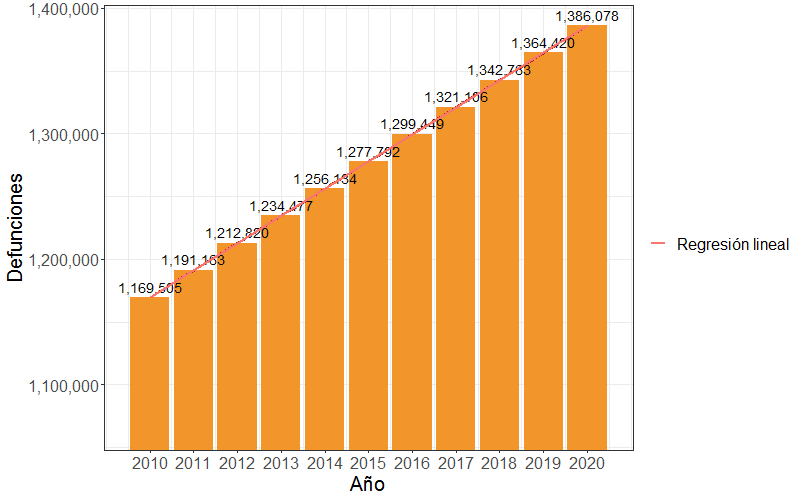
\includegraphics[width=0.6\textwidth]{Figuras/DefuncionesAnualesRegresionFinalBrasil.png}}%
\hfill
\caption{Regresión lineal para el país de Brasil junto con la media en 2020.}

\label{fig:RegresionBrasil}
\end{figure}   
\hfill


\section{Conclusión}

Para el caso de Brasil y los Estados Unidos, los resultados muestran una pequeña inconsistencia sin embargo la regresión puede ser un muy buen dato, para Canadá la regresión lineal no parece ser la mejor forma de calcular el valor estimado pues los valores parecen llevar una tendencia al alza, por lo que nuestro valor quedaría un poco corto, para el caso específico de México también la regresión lineal no se muestra muy confiable, especialmente por el último año en donde las muertes parecen haberse disparado, esto puede ser debido al aumento de muertes por asesinatos, por lo que esperamos que el valor estimado de muertes seria el límite superior de nuestro intervalo. Se ha reportado que en México el número de muertes por accidentes también ha aumentado este año 2020 por lo que sería también conveniente hacer la comparación con el número de muertes eliminando este dato de la cifra total de muertos, pudiendo de esta manera, obtener el número de muertes en exceso que pudo haber causado el Covid en 2020, en México y en los otros países.
Solo faltaría comparar con el dato final que se publica hasta en Marzo de 2021, actualmente el Covid se convirtió en la causa número 2 en México en 2020.

\printbibliography[title={Referencias}]
\end{document}
